\chapter{Agradecimientos}

¿Qué se siente cuando uno echa la vista atrás? ¿Qué es lo que se te pasa por la cabeza antes de pasar la última página de un libro que te ha tenido atrapado horas y horas? ¿Qué queda cuando, en la cima de la montaña, miras hacia arriba solamente para descubrir que todo queda bajo tus pies? Todas las historias acaban de alguna forma o de otra y todo lo que queda cuando lo hacen es el vacío de saber que nunca jamás nada podrá reemplazarlas, ni tan siquiera acercarse a ellas. Es la ineludible sensación de todo aquello que al final del camino ha merecido la pena.

Este documento recoge de forma académica la historia de los mejores seis años de mi vida. Detrás de todos los tecnicismos se encuentra la historia de más de veinte ciudades; de no menos de sesenta vuelos, trenes y coches; y lo más importante: de por lo menos cien personas. Desafortunadamente, no creo que ningún editor con dos dedos de frente decidiera publicar semejante despropósito, de modo que aprovecharé estas páginas que serán publicadas sin revisión para contar mi vida.

Como todo niño fascinado por el espacio, soy un astronauta frustrado. Uno que no tuvo la valentía de moverse y estudiar Física y que por suerte tenía unas manos demasiado sudorosas como para dedicarse a la Arquitectura. El metro ochenta de mi niñez me hizo buen jugador de baloncesto hasta que todo el mundo creció. La portería de fútbol, que será siempre el lugar donde me sienta la persona más importante del Universo, era a la vez demasiado solitaria para mí. Toqué el piano sin brillantez. Pinté sin genialidad. Escribí, publicado, pero escaso de tinta y de imaginación. Diseñé y construí puentes, pero solo de palillos de helado. Probé muchas cosas y tuve la suerte de encontrar mi ikigai en la informática. Supongo que en el momento en el que instalé mi primera tarjeta gráfica y ejecuté \verb|C:\>DOOM\doom.exe| todo quedó sellado. Jamás imaginé que aquel chaval que simplemente quería hacer un videojuego divertido acabaría pasando incontables horas devorando todo el conocimiento que encontrara a su paso sobre programación, estructuras de datos y algoritmos.

Así pues, como toda mi generación, entré en la Universidad con la promesa de un empleo y una vida digna ganada gracias al estudio. Transcurrieron así los mejores momentos de mi vida entre partidas de futbolín, preocupaciones y caras de sueño antes de entrar a clase, risas al salir de ellas y noches de partidas eternas de League of Legends y Counter Strike. Nada tiene que ver la persona que entró (cerrada, de frases cortas y sonrisas escasas) con la que salió (decidida, locuaz y risueña). De paso, conseguí vestirme de una manera algo más decente, aunque sigo sin encontrar la manera de combinar colores con acierto. En esos cuatro años conocí a un grupo de personas excepcionales, aprendí y estudié hasta el más mínimo detalle, me encontré con quienes serían mi guía en los años venideros y descubrí que la investigación era mi misión en la vida.

Al terminar, volé por primera vez por mi cuenta hacia el Centro de Supercomputación de Jülich (Alemania) para lo que sería mi primera estancia fuera. Fueron sin lugar a dudas el momento más trasdencental en mi vida. Tan buen recuerdo guardo de aquellas semanas que nunca quise volver por no estropearlo. Como diría el maestro Sabina: "[...] que al lugar donde has sido feliz, no debieras tratar de volver [...]".

Más por inercia e ilusión que por lógica, decidí estudiar un máster en Robótica en mi alma mater. Siendo sinceros, no fue la alternativa más inteligente para mi futuro. Sencillamente, con el paso del tiempo me di cuenta de que en el fondo siempre me arrepentiré de no haber subido a un avión para descubrir otra Universidad. Sin embargo, de no haberme quedado, jamás habría conocido tanto ni hubiera trabado amistad con una de las mejores personas que se han cruzado en mi vida. Cada vez que pienso en que tendría que haber volado, le recuerdo comiendo un limón entero con piel y se me pasa.

Como si de alguna forma se escucharan mis lamentos, la vida me dio la oportunidad inmejorable de volar hacia los Estados Unidos e investigar en una de las compañías a las que más cariño guardaré. Así acabé viviendo en Mountain View (California) y trabajando para NVIDIA con un equipo excepcional. Fueron meses de descubrimiento en todos los sentidos y quedarán para siempre en mi memoria los recuerdos de mi pequeña habitación en Villa Street, del conductor de autobuses al que nunca le pregunté su nombre pero que siempre me llevaba con una sonrisa al trabajo y un "Hey, buddy!", de las partidas de ping pong después de comer, del DeLorean aparcado delante de mi casa y de disfrutar de los Juegos Olímpicos en el proyector de la casa de Cole gritando "USA, USA, USA!". La hospitalidad de Cole y Grayson hicieron que esos meses se me pasaran volando.

\newpage

Como el hombre es el único animal que tropieza dos veces con la misma piedra, regresé de nuevo a Alicante a comenzar mi doctorado. De nuevo, uno de mis mayores defectos me jugaba una mala pasada y nublaba mi juicio al elegir: la comodidad. De nuevo, siempre quedará en mi cabeza la incógnita de qué hubiera ocurrido si hubiera decidido quedarme en Estados Unidos en lugar de volar de vuelta. De nuevo, como si algún desconocido bondadoso me ayudara a llevar una carga pesada, la vida se encargaría de darme una palmada en la espalda y recordarme que no fue tan mala elección. Apenas unas semanas después de mi vuelta, quizás movido por la confianza insuflada por todo lo conseguido, quizás guiado por la inconsciencia etílica, envié un mensaje que me permitió conocer a la persona que me ha dado todo lo que me faltaba en la vida. Como un Tetris perfecto, todas las piezas empezaron a caer en su sitio: con la guía y el empuje de mis directores (más amigos que jefes) y con el regreso de viejos compañeros formamos un equipo con el que con mucho esfuerzo conseguimos empujar mínimamente la frontera del conocimiento pero con el orgullo del trabajo bien hecho pese a todos los obstáculos. De nuevo, con la fortuna sonriendo, partí una vez más hacia Estados Unidos a trabajar con una de las personas que más admiraba desde que comencé mis andaduras. Fue un otoño complicado, con mi cabeza más dispersa que nunca y marché con la sensación de no haber hecho todo lo que estaba en mi mano.

Esa cabeza dispersa pasó unos cuantos meses más perdida y con la sensación de estar desperdiciando el tiempo. La inevitable comparación con todo el mundo alrededor del globo no era favorable. Las experiencias vividas, si bien enriquecedoras, eran un arma de doble filo capaces de minar la confianza en uno mismo al darse cuenta de todo el talento y la gente excepcional que trabaja sin cesar fuera. La perspectiva del fin de la etapa añadía todavía más si cabe un componente de incertidumbre que se transformó en sueño escaso, irritabilidad, desmotivación y pesimismo. Me convertí en mi propio peor enemigo, incapaz de sentirme satisfecho con el pasado, completamente ajeno del presente y ciego de cara al futuro. Avanzando a rastras, buscando refugio en todos los hobbies existentes (muchos de los cuales se acabaron convirtiendo en una decoración fantástica para mi habitación) y únicamente espoleado por los estudios paralelos en Física y por el aliento de los seres queridos para continuar, comencé a escribir el documento que aquí presento.

\newpage

Fue justo en el momento de mayor desánimo en mi carrera cuando ocurrió algo completamente inesperado que lo cambió todo. Sin ninguna gana ni motivación, partí hacia Zürich a pasar los meses de verano en la que sería mi última estancia, de nuevo en Oculus. En el momento en el que más lo necesitaba, todos los astros se alinearon para ofrecerme una ciudad y una casa fantásticas, un equipo de gente extremadamente capaz y amigable, un mentor atento y comprensivo... y un grupo de gente de mi tierra tremendamente afín con el que compartir absolutamente todo. Gracias a ello recuperé la motivación y la ilusión para seguir adelante y poder escribir estas líneas.

Como podéis leer, ha sido un camino curioso y lleno de subidas y bajadas. Esta montaña rusa emocional me ha costado pelo, horas de sueño, discusiones y muchos arrepentimientos. Sin embargo, ahora en pie desde la cima de la montaña, observando mi vida a vista de pájaro puedo decir que no hubiera cambiado nada. He recorrido mi propio camino toda la honestidad e integridad que he podido, he volcado todo el esfuerzo que mi salud mental me ha permitido y he tratado de ser la mejor versión de mí mismo a cada paso dado. En algunas ocasiones habré acertado y en otras habré fracasado, pero este ha sido el camino que yo he trazado y eso es algo que recordaré con cariño toda la vida.
Ante mi vista se extienden ahora innumerables cumbres que antes jamás hubiera podido divisar ocultas por las nubes a gran altura. Aquí planto mi bandera y me siento a agradecer a todas aquellas personas que de alguna forma o de otra me han permitido llegar hasta aquí.

Gracias a todos aquellos profesores que se esforzaron en su día a día lleno de complicaciones para que sus alumnos aprendieran y que día a día nos demostraron su cariño y su implicación. Estoy seguro de que si alguno de vosotros tanto del Colegio Sagrada Familia como del Colegio El Valle leéis estas líneas os sentiréis identificados y van por vosotros. En concreto, quiero dedicar unas líneas a agradecer a una persona excepcional que tendrá siempre mi más profunda admiración: Don Carlos. Más allá de enseñarnos, supo transmitirnos pasión, autenticidad y cariño hasta en los días más difíciles. No puedo olvidarme tampoco de Don Francisco, de quien aprendí la importancia del lenguaje; si algún día escribo una novela, será culpa suya.

\begin{center}
\includegraphics[width=0.45\linewidth]{Figures/Ack/valle}
\includegraphics[width=0.45\linewidth]{Figures/Ack/valle2}
\end{center}

Gracias a todos los profesores universitarios que, rodeados de incompetencia, obstáculos y desgana, siguieron dando todo lo que tenían para mantener la educación pública en el lugar que se merece. Aprovecho estas líneas para agradecer a José Miguel Torrejón por demostrarnos que lo difícil se puede hacer fácil con la explicación adecuada y por tener siempre su puerta abierta para cualquier curiosidad. De la misma manera a José Pons, por hacer todo lo que estuviera en su mano para que pudiera formarme en Física y ofrecerme una nueva oportunidad que explorar.

Gracias a todos aquellos que fueron mi guía durante mi etapa investigadora. A Higinio porque realmente él es el responsable de que me dedicara a investigar, gracias por tu franqueza, dedicación y sinceridad.

A Jose, por acogerme y tratarme siempre como un amigo; aunque no hayas estado en la arena, has peleado por mí y siempre has tratado de buscar lo mejor para mi futuro incluso cuando lo mejor para mí no era lo mejor para ti; no has sido mi director, has sido mi amigo y padre académico.

A Sergio, porque sin él todo lo conseguido hubiera sido directamente imposible; has estado con todos nosotros siempre al pie del cañón no importa cuándo ni dónde, has sido el pegamento que nos ha mantenido unidos, el espejo en el que todos nos hemos querido mirar y la fuente de inspiración que nos ha empujado a todos a ser mejores cada día.

\begin{center}
	\includegraphics[width=0.6\linewidth]{Figures/Ack/sergio}
\end{center}

A Ivo, porque su energía es contagiosa y su optimismo incansable.

A mi mánager y mentores en NVIDIA, Howard, Bryan y Shalini, por todo el tiempo que me dedicasteis y el buen trato que recibí de vosotros. A todos los integrantes de NVIDIA Research y del equipo de Camera Solutions por compartir tanto conocimiento y consejos: Orazio, Kihwan, Jinwei, Pavlo, Jan, Vidya, Dhaval y John. A todos los interns que compartimos tantos buenos ratos, preocupaciones y naps: Suren, Robert, Behrooz, Zhaopeng y Abhishek.

\begin{center}
\includegraphics[width=0.44\linewidth]{Figures/Ack/nvidia}
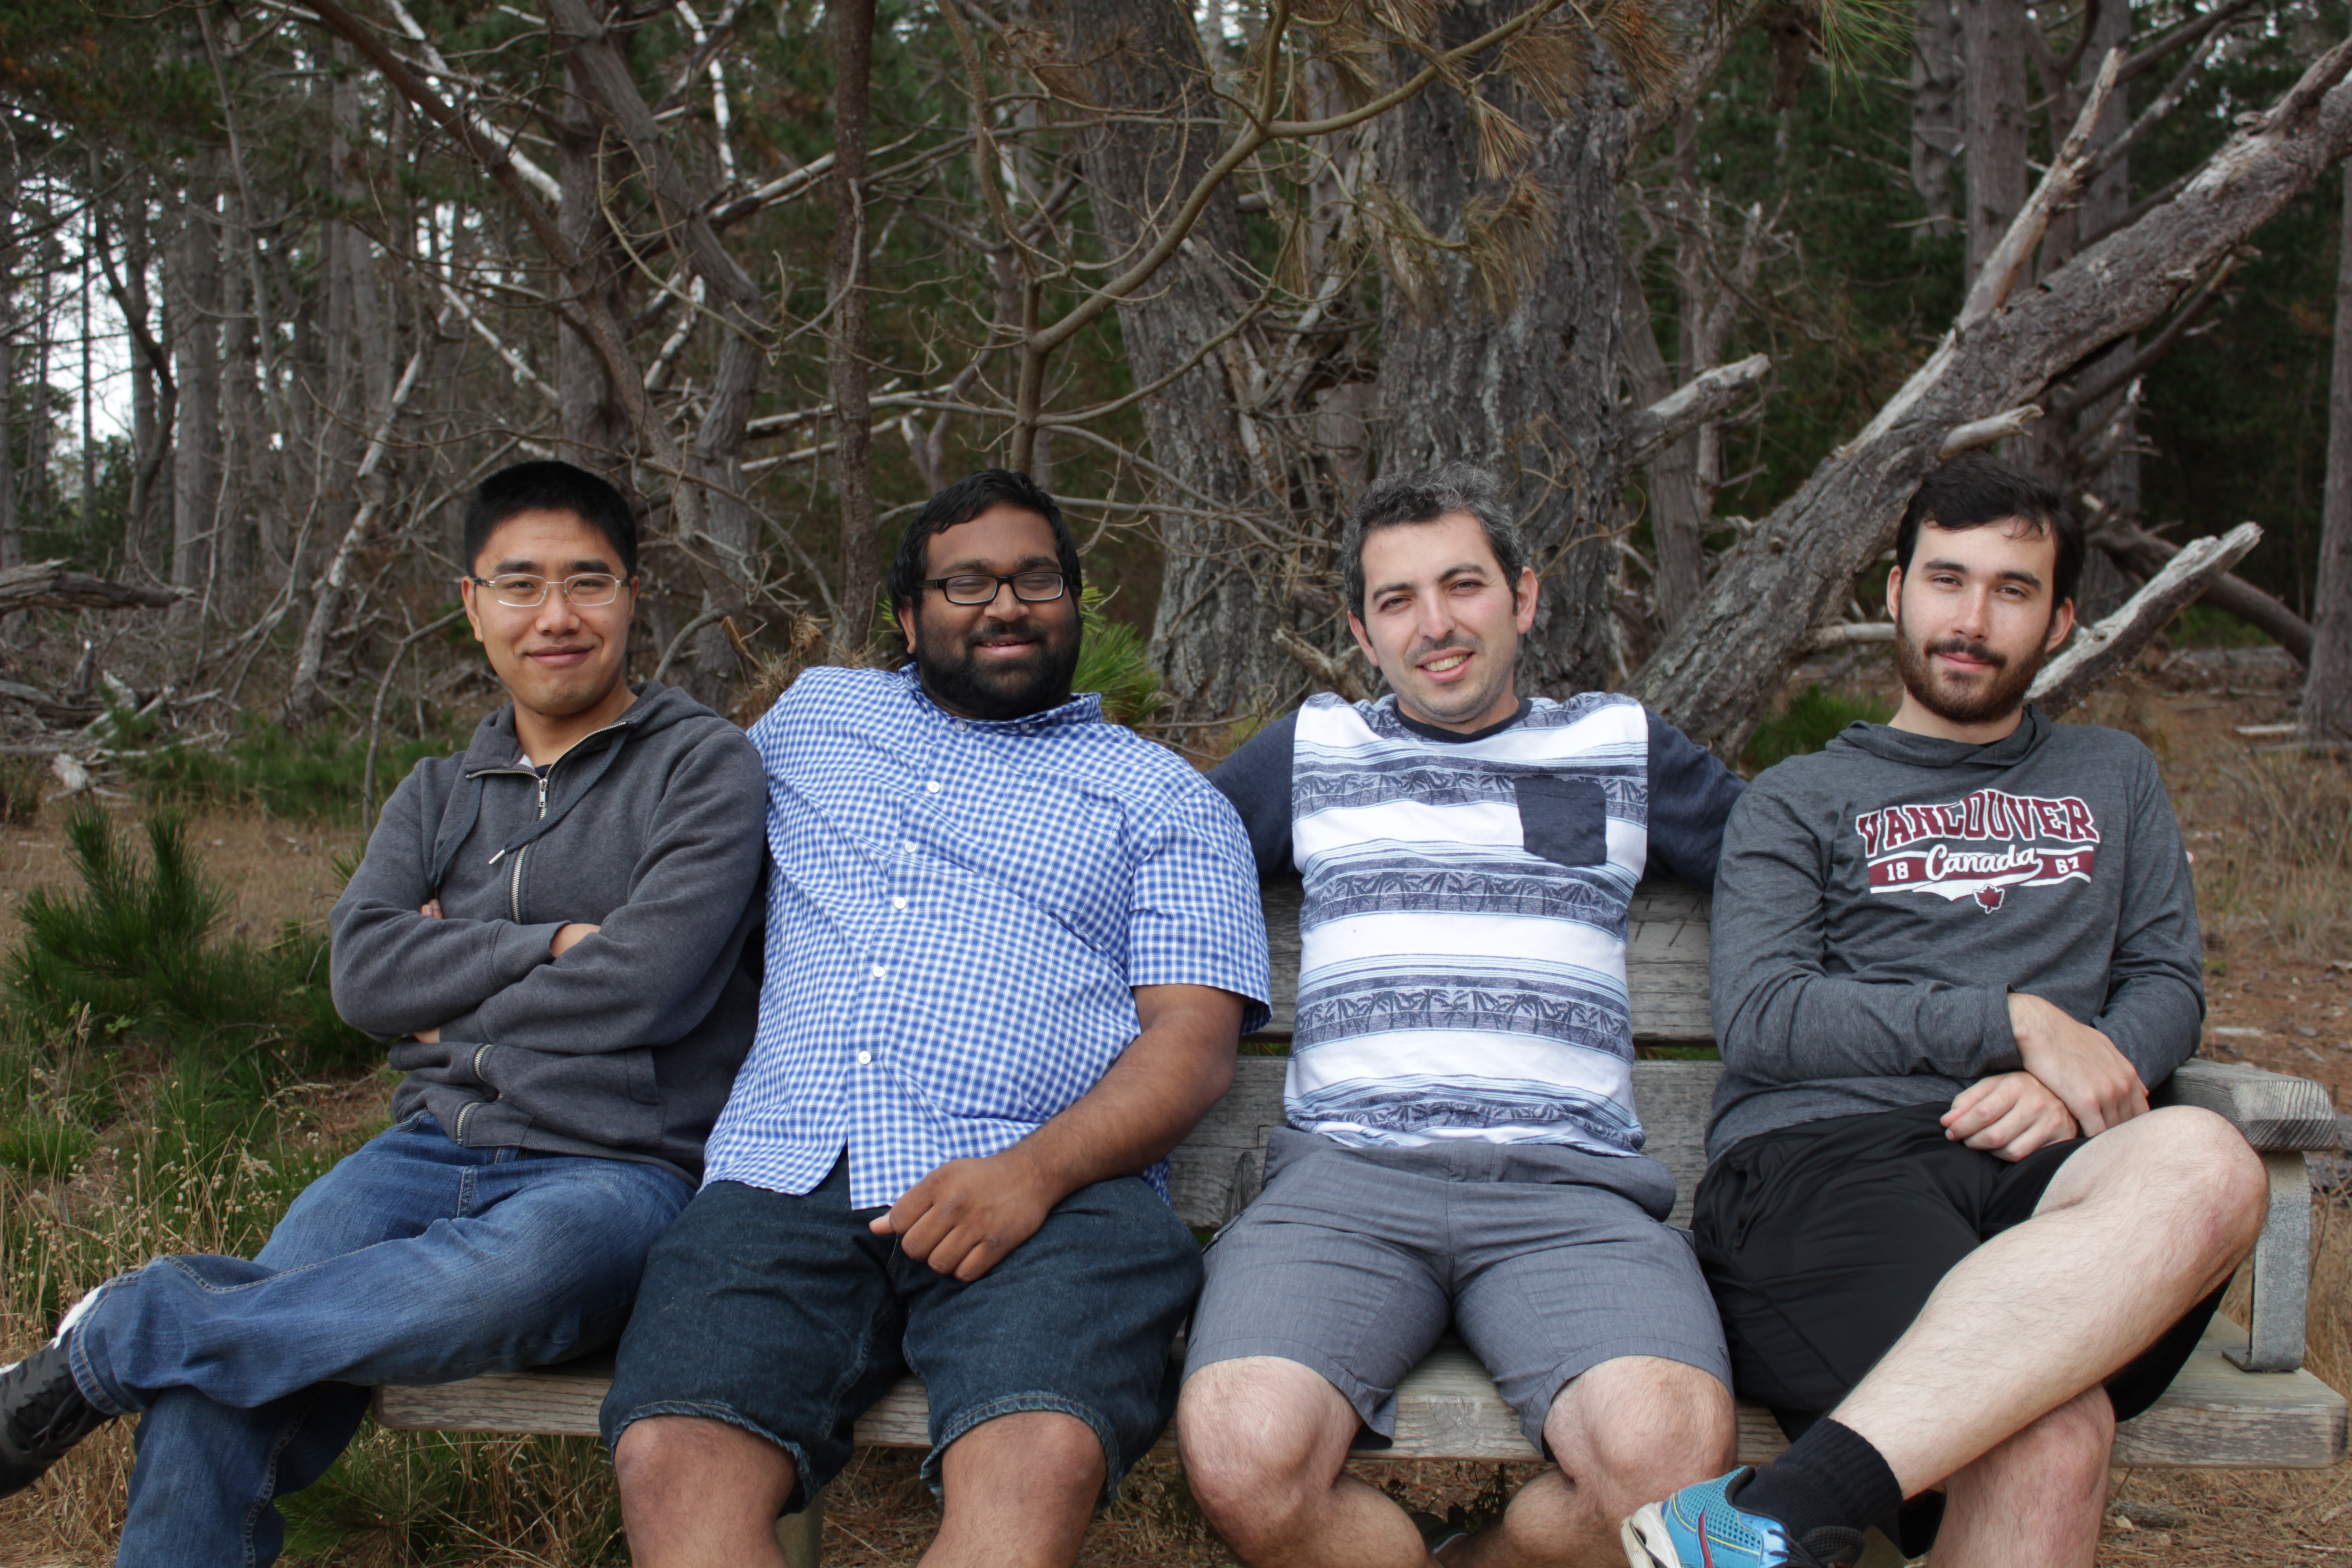
\includegraphics[width=0.5\linewidth]{Figures/Ack/nvidia2}
\end{center}

A mi mentor durante mi estancia en Facebook Reality Labs, Richard Newcombe, para mí fue alucinante poder compartir ideas con alguien al que admiraba tanto, gracias por hacer un hueco en tu agenda. A Raúl por hacerme más llevadera la estancia. A Lingni por tener tanta paciencia conmigo, jamás he visto a alguien que trabaje tan duro. A Svet por sus archivos de calibración. A los demás compañeros del equipo Surreal y Oculus Research que me hicieron sentirme como en casa: Nikki, Theo, Julian, Carl, Tom y Steve.

\begin{center}
\includegraphics[width=0.6\linewidth]{Figures/Ack/frl2}
\end{center}

A los alumnos con los que he tenido el placer de compartir algunas horas. Gracias por darme vuestra atención y cariño. Nunca imaginé que disfrutaría tanto de la docencia pero os puedo asegurar que con vosotros en el aula he compartido algunos de los momentos en los que me he sentido más lleno en la vida. En especial, gracias a todos los que decidisteis invertir vuestro tiempo conmigo haciendo vuestro TFG o prácticas: Álvaro, Adri, Alexei, Iván, Plácido, Mario, David y Pablo. Vuestra curiosidad y empuje me hacían tener ganas de veros cada día. Espero que todos consigáis todo lo que os propongáis y lo compartáis conmigo allá donde andéis.

\begin{center}
\includegraphics[width=0.64\linewidth]{Figures/Ack/tfg1}
\end{center}

A todos los personajes célebres que han pasado por el laboratorio y que de alguna forma o de otra han aportado su granito de arena para hacer los días diferentes: Rafa, Marcelo, Jose María, Luis, Vicente, Alexandros, Zuri, Isaza, Alejandro, Pau, Toni, Jose Manuel... Y a Joan Carles por dar de alta mi dirección MAC y enseñarme a jugar al pádel.

\begin{center}
	\includegraphics[width=0.75\linewidth]{Figures/Ack/dtic1}
\end{center}

A todos los compañeros inolvidables que he tenido el placer y la suerte de conocer durante la carrera, en el preciso orden en el que saludé a cada uno de ellos: Manu, 0xthor, Pajarraco, Mmarinero, Pable, Víctor, Ginés, Caye y por último y no menos importante, Brayan. Jamás en la vida volveré a encontrar un grupo de gente con la que compartir tantas aficiones, risas, cafés, noches en vela y rusheos por B. Todo lo que pudiera escribir aquí se quedaría corto.

\begin{center}
	\includegraphics[width=0.5\linewidth]{Figures/Ack/bsc1}
\end{center}

A Víctor y a Fran

\emph{Zurich}

A mi hermano, porque aunque no hayamos tenido la mejor ni la más intensa de las relaciones, siempre se ha alegrado de todo lo que he conseguido y yo siempre estaré orgulloso de lo que él alcance.

A mis padres porque lo han dado todo para que nunca nos faltara de nada. Porque todo lo que ha estado en su mano ha sido para nosotros en lugar de para ellos. Porque siempre nos han tratado con cariño y comprensión. Porque gracias a ellos he podido ser todo lo que he querido.

A Carol, porque apareció justo en el momento perfecto y yo no creo en las coincidencias. Ella ha soportado todo lo malo de este camino y lo ha amortiguado, ha recibido todo lo bueno y lo ha potenciado. Han sido muchos momentos difíciles para los dos en todos los sentidos y hemos compartido todas las preocupaciones e inquietudes que se le pueden pasar a uno por la cabeza. Han sido también los años más intensos de mi vida gracias a ti. No sé lo que nos deparará la vida, pero siempre tendrás un hueco en mi corazón. Eres la mejor compañera de viaje que uno puede imaginar.\\

\emph{Alberto García García}\\
\emph{Septiembre de 2019}\\
\emph{Zürich}\\

\chapter{Acknowledgements}

\lipsum[3]
\lipsum[2]
\lipsum[4]
\lipsum[5]
\lipsum[6]
